\section{RAVEN Theory by way of Examples: Data Mining}

Data mining is the computational process of discovering patterns in large data sets (``big data'') involving methods at the intersection of artificial intelligence, machine learning, statistics, and database systems. The overall goal of the data mining process is to extract information from a data set and transform it into an understandable structure for further use.
\\RAVEN has support of several different data mining algorithms,
such as:
\begin{enumerate}
  \item \textit{Hierarchical methodologies}
  \item \textit{K-Means}
  \item \textit{Mean-Shift}, etc.
\end{enumerate}
In this section only few algorithms will be analyzed, explaining the theory behind them
by way of applied RAVEN examples.

\subsection{Data Mining Theory}
\label{sec:dataMining}

\subsubsection{Clustering}
\label{clustering}
A loose definition of clustering is the process of organizing objects into groups whose members are, in some way, similar.
Therefore, a cluster is a collection of objects that are similar to each other and are dissimilar to the objects belonging to other clusters~\cite{SurveyClustering,MandelliClusteringRESS}.

The similarity criterion is distance. Two or more objects belong to the same cluster if they are ``close'' according to a specified distance. The approach of using distance metrics to clustering is called distance-based clustering and is used in this work.

The notion of distance implies that the data points lay in a metric space \cite{Mendelson75introduction}:

    \begin{mydef}[Metric Space]
    A metric space is a space X provided with a function \emph{d}:
    \begin{math}
    f: X\times X\rightarrow \mathbb{R}
    \end{math}
    satisfying the following properties \begin{math}\forall \vec{x},\vec{y} \in X \end{math} :

    \begin{itemize}
      \item \begin{math} d(\vec{x},\vec{y}) \geqslant 0 \end{math}
      \item \begin{math} d(\vec{x},\vec{y}) = d(\vec{y},\vec{x}) \end{math}
      \item \begin{math} d(\vec{x},\vec{y}) \leqslant d(\vec{x},\vec{z}) + d(\vec{z},\vec{y}) \end{math}
    \end{itemize}

    \end{mydef}

The function \begin{math} d(\vec{x},\vec{y}) \end{math} is usually called the distance function. In a 2-dimensional Euclidean space ($\mathbb{R}^{2}$), the distance between points can be calculated using the Pythagorean theorem which is the direct application of the Euclidean distance and is a special case of the most general Minkowski distance \begin{math}\ d_{2}(\vec{x},\vec{y}) = \sqrt{(x_{1}-y_{1})^{2}+(x_{2}-y_{2})^{2}} \end{math} between two points $\vec{x}=(x_{1},x_{2})$ and $\vec{y}=(y_{1},y_{2})$ in $\mathbb{R}^{2}$.

In the literature~\cite{Mendelson75introduction}, it is possible to find several types of distances other than the Euclidean and the Minkowski distance as shown in Table~\ref{table:tableDist}. The approach of using distance metrics is called distance-based clustering and will be used in this dissertation.

    \begin{table}[ht]
    \caption {\small Summary of the commonly used measures \cite{Mendelson75introduction}.}
    \centering
    \begin{tabular}{c c }
    \hline\hline
    Measure & Form \\ [0.5ex]
    \hline
    \hline
    Minkowski distance & \begin{math}\ d_{n}(\vec{x},\vec{y}) = (\displaystyle \sum_{k=1}^\delta |x_{k}-y_{k}|^{n})^{\frac{1}{n}} \end{math} \\
    Euclidean distance & \begin{math}\ d_{2}(\vec{x},\vec{y}) = (\displaystyle \sum_{k=1}^\delta |x_{k}-y_{k}|^{2})^{\frac{1}{2}} \end{math} \\
    Taxicab distance & \begin{math}\ d_{1}(\vec{x},\vec{y}) = \displaystyle \sum_{k=1}^\delta |x_{k}-y_{k}| \end{math} \\
    Supremum distance & \begin{math}\ d_{0}(\vec{x},\vec{y}) = \displaystyle max_{k} |x_{k}-y_{k}| \end{math} \\
    Mahalanobis distance & \begin{math}\ d_{M}(\vec{x},\vec{y}) = (\vec{x}-\vec{y})^{T} S^{-1} (\vec{x}-\vec{y}) \end{math} \\
    \hline
    \end{tabular}
    \label{table:tableDist}
    \end{table}

From a mathematical viewpoint, the concept of clustering~\cite{SurveyClustering} aims to find a partition $\mathbf{C}=\{C_{1},\ldots,C_{l},\ldots,{C_{L}}\}$
of the set of $I$ scenarios
    $\mathbf{X} = \{\vec{x_{1}},\ldots,\vec{x_{i}},\ldots,\vec{x_{I}}\}$
where each scenario $\vec{x_{i}}$ is represented as a $\delta$-dimensional vector.
Each $C_{l}$ $(l=1,\ldots,L)$ is called a cluster. The partition
    $ \mathbf{C} $ of $ \mathbf{X} $
is given as follows\footnote{In most clustering algorithms each scenario belongs to only one cluster. However this is not always the case. In fuzzy clustering methodologies~\cite{ZioMaio} a scenario may be allowed to belong to more than one cluster with a degree of membership
\begin{math} u_{i,j}\in [0,1] \end{math} which represents the member coefficient of the $j$ scenario for the $i^{th}$ cluster and satisfies the following properties:

$ \sum_{i=1}^{K}u_{i,j}=1,  \text{ and }  \sum_{j=1}^{N}u_{i,j}<N, \forall j $}:

    \begin{equation}\label{eq: ClassRequier}
        \begin{cases} \mathbf{C}_{l}\neq\varnothing, l=1,\ldots,L \\
                        \\
                     \bigcup_{l=1}^{L}\mathbf{C}_{l}= \mathbf{X} \\
        \end{cases}
    \end{equation}

\subsubsection{Hierarchical Methodologies}
\label{Hierarchical}

These methodologies organize the data set into a hierarchical structure according to a proximity matrix. Each element $d(i,j)$ of this matrix contains the distance between the the $i^{th}$ and the $j^{th}$ cluster center. The final results of this technique is a tree commonly called a dendrogram. This kind of representation has the advantages of providing a very informative description and visualization of the data structure even for high values of dimensionality.

The procedure to determine the dendrogram for a data set of $I$ points in an $\delta$-dimensional space is the following:

\begin{enumerate}
  \item Start the analysis with a set of $I$ clusters (i.e., each point is considered as a cluster).
  \item Determine the proximity matrix $M$ (dimension: $I\times I$): $M(i,j)= d(\vec{x_{i}},\vec{x_{j}})$ where $\vec{x_{i}}$ and $\vec{x_{j}}$ are the position of the $i^{th}$ and the $j^{th}$ cluster.
  \item For each point $p$ find the closest neighbor $q$  from the proximity matrix $M$
  \item Combine the points $p$ and $q$
  \item Repeat Steps 2, 3 and 4 until all the points of the data set are in the same cluster
\end{enumerate}

The advantage of this kind of algorithm is the nice visualization of the results that show the underlying structure of the data set. However, the computational complexity for most of the hierarchical algorithm is of the order of $\mathcal{O}(I^{2})$ (where \emph{I} is the number of points in the data set).

\subsubsection{\emph{K}-Means}
\label{KMeans}

\emph{K}-Means clustering algorithms belong to the more general family of Squared Error algorithms. The goal is to partition $I$ data points $\vec{x_{i}}$ $(i=1,\ldots,I)$ into \emph{K} clusters in which each data point maps to the cluster with the nearest mean. The stopping criterion is to find the global minimum of the error squared function $\chi$ defined as:

\begin{equation}
    \chi = \displaystyle \sum_{i=1}^K \displaystyle \sum_{x_{j}\in C_{i}} |\vec{x_{j}}-\vec{\mu_{i}}|^{2}
\end{equation}

where $\vec{\mu_{i}}$ is the centroid (i.e., the center) of the cluster $C_{i}$.

The procedure to determine the centroids $\vec{\mu_{i}}$ of \emph{K} clusters (${C_{1},\ldots,C_{K}}$) is the following:

\begin{enumerate}
  \item Start with a set of $K$ random centroids distributed in the state space
  \item Assign each pattern to the the closest centroid
  \item Determine the new $K$ centroids according to the point-centroid membership

    \begin{equation}
        \mu_{i} = \displaystyle \frac{1}{N_{i}} \sum_{\vec{x_{j}}\in C_{i}} \vec{x_{j}}
    \end{equation}

    where $N_{i}$ corresponds to the number of of data points in the $i^{th}$ cluster.

  \item Repeat Steps 2 and 3 until convergence is met (i.e., until a minima of the $\chi$ function is reached)
\end{enumerate}

\emph{K}-Means algorithm is one of the most popular and used methodologies also due to the fact that is very straightforward to implement and the computational time is directly proportional to the cardinality of data points (i.e., $\mathcal{O}(I)$ where \emph{I} is the number of data points). The main disadvantage is that the algorithm is sensitive to the choice of the initial partition and may converge to a local minimum of the error squared function~\cite{JainAlgor88}. Another disadvantage of this algorithm is that is only able to identify clusters having spherical or ellipsoidal geometry. Thus, \emph{K}-Means is not able to identify clusters of points having arbitrary shapes. Moreover, the number of cluster \emph{K} to be obtained is specified by the user prior the clustering process.

%\subsubsection{Fuzzy C-Means}
%\label{FuzzyCMeansn}
%
%Fuzzy \emph{C}-Means clustering is a clustering methodology that is based on fuzzy sets and, hence, it allows a data point to belong to more that one cluster~\cite{FuzzyBezdek,DunnFuzzy}. Similar to the \emph{K}-Means clustering, the objective is to find a partition of $C$ fuzzy centers to minimize the function $J$ defined as following:
%
%\begin{equation}
%    J = \displaystyle \sum_{i=1}^I \displaystyle \sum_{j=1}^C u_{ij}^{m}|\vec{x_{i}}-\vec{\mu_{j}}|^{2}
%\end{equation}
%
%where:
% \begin{itemize}
%   \item $u_{ij}^{m}\in[0,1]$ is the membership coefficient of the data point $\vec{x_{i}}$ for the $j^{th}$ cluster having centroid $\vec{\mu_{j}}$,
%   \item $m\in[0,\infty)$ is the fuzzification parameter (usually set to $m=2$), and,
%   \item $\mu_{j}$ is the centroid of the $j^{th}$ cluster center
% \end{itemize}
%
%The procedure to determine the centroids (or, equivalently, cluster centers)
%$ \vec{\mu_{j}}$ $(j=1,\ldots,C)$ of $C$ clusters is the following:
%
%\begin{enumerate}
%  \item Initialize the $U=[u_{ij}^{m}]$ matrix
%  \item Calculate the set of $C$ centroids  as following:
%
%          \begin{equation}
%            \mu_{j}=\frac{\sum_{i=1}^N u_{ij}^{m}x_{i}}{\sum_{i=1}^N u_{ij}^{m}}
%          \end{equation}
%
%  \item Update the matrix $U=[u_{ij}^{m}]$ as following:
%
%          \begin{equation}
%            u_{ij}^{m}=\frac{1}{\sum_{k=1}^C (\frac{|x_{i}-\mu_{j}|}{|x_{i}-\mu_{k}|})^{\frac{2}{m-1}}}
%          \end{equation}
%
%  \item Repeat Steps 2 and 3 until convergence, i.e. if \begin{math} |U^{(K+1)}-U^{(K)}|<\epsilon \end{math}
%\end{enumerate}
%
%Fuzzy \emph{C}-Means clustering is very similar to the \emph{K}-Means. As seen for the \emph{K}-Means, Fuzzy \emph{C}-Means can also converge to a local minima of the convergence criterion function~\cite{FuzzyBezdek}.
%Like \emph{K}-Means, it is not able to identify cluster of points having arbitrary shapes but only clusters having ellipsoidal or spherical geometry and the number of clusters \emph{C} to be obtained is specified by the user prior the clustering process.
%Fuzzy \emph{C}-Means algorithms can be useful when the boundaries among clusters are ambiguous and not well defined.

\subsubsection{Mean-Shift}
\label{Mean-Shift}

The Mean-Shift algorithm~\cite{EstimationGradient} is a non-parametric iterative procedure that can be used to assign each point to one cluster center through a set of local averaging operations~\cite{EstimationGradient}. The local averaging operations provide empirical cluster centers within the locality and define the vector which denotes the direction of increase for the underlying unknown density function.

The underlying idea is to treat each point $\vec{x_{i}}$ $(i=1,\ldots, I)$ of the dataset as an empirical probability distribution function using  kernel $K(\vec{x}): \mathbb{R}^{M\cdot K}\rightarrow \mathbb{R}$. This multivariate kernel density resides in a multidimensional space where regions with high data density (i.e., modes) correspond to local maxima of the density estimate $f_{I}(\vec{x})$~\cite{CacoullosEstimation}  defined by:
\begin{equation}
    f_{I}(\vec{x})=\frac{1}{Ih^{d}}\sum_{i=1}^{I} K\left(\frac{\vec{x}-\vec{x_{i}}}{h}\right),
    \label{eq:density:estimate}
\end{equation}
where $\vec{x}\in \mathbb{R}^{M\cdot K}$ and $h$ is often referred as the bandwidth associated with the kernel.

The kernel in Equation ~\ref{eq:density:estimate} serves as a weighting function~\cite{CacoullosEstimation} associated with each data point and is expressed as:
\begin{equation}
    K(\vec{x})=c_{k} k(\norm{\vec{x}}^{2})
\end{equation}
where $k(x):[0,\infty]\rightarrow \mathbb{R}$ is referred as the \emph{kernel profile} and $c_{k}$ is a normalization constant. The profile satisfies the following properties:
\begin{itemize}
  \item $k(x)$ is non negative
  \item $k(x)$ is non increasing (i.e., $k(a)\geq k(b)$ if $a<b$)
  \item $k(x)$ is piecewise continuous and $\int_0^\infty \! k(x) \, dx < \infty$
\end{itemize}

In order to estimate the data points with highest probability from an initial estimate (i.e., the modes of $f_{I}(\vec{x})$), consider the gradient of the density function $\nabla_{x} f_{I}(\vec{x})=0$ ~\cite{EstimationGradient} where
\begin{eqnarray}
\label{gradient}
    \nabla_{x} f_{I}(\vec{x}) & = & \frac{2 c_{k}}{I h^{d+2}} \sum_{i=1}^{I}(\vec{x}-\vec{x_{i}})k'\left(\norm{\frac{\vec{x}-\vec{x_{i}}}{h}}^{2}\right) \nonumber \\
    & = & \underbrace{\frac{2 c_{k}}{I h^{d+2}} \left(\sum_{i=1}^{I} g\left(\norm{\frac{\vec{x}-\vec{x_{i}}}{h}}^{2}\right)\right)}_{A}
    \underbrace{\left(\frac{\sum_{i=1}^{I}
    \vec{x} g\left(\norm{\frac{\vec{x}-\vec{x_{i}}}{h}}^{2}\right)}{\sum_{i=1}^{I} g\left(\norm{\frac{\vec{x}-\vec{x_{i}}}{h}}^{2}\right)}-\vec{x}\right)}_{B},
\end{eqnarray}
which points in the direction of the increase in kernel density estimate. The kernel $K(\vec{x})$ is also referred to as the shadow of $G(\vec{x})=c_{g} g(\norm{\vec{x}}^{2})$~\cite{Mode-seekingMedoidshifts} where $c_{g}$, similar to $c_{k}$, is a normalization constant and $g(x)$ is the derivative of $k(x)$ over $x$, i.e., $g(x)=k'(x)$. In the equation above, the first term denoted as $A$ is a scalar proportional to the density estimate computed with the kernel $G(\vec{x})$ and does not provide information regarding where the mode resides. Unlike $A$, the vector quantity $B$, which is the second term in the equation above, is difference between the weighted mean
\begin{equation}
	m(\vec{x})=\frac{\sum_{i=1}^{I}\vec{x} g(\norm{\frac{\vec{x}-\vec{x_{i}}}{h}}^{2})}{\sum_{i=1}^{I} g(\norm{\frac{\vec{x}-\vec{x_{i}}}{h}}^{2})}.
\end{equation}

and the initial estimate $\vec{x}$. This term points in the direction of local increase in density using kernel $G(\vec{x})$, hence provides a means to find the mode of the density. Note that all points used to compute a particular mode are considered to reside in the same cluster.

Since each each data point $\vec{x_{i}}$ (or scenario) is considered as an empirical probability distribution function, this consideration allows to include in the scenario clustering analysis also the possible uncertainty associated with each scenario.

\subsubsection{DBSCAN }
\label{DBSCAN }

The Density-Based Spatial Clustering of Applications with Noise (DBSCAN) algorithm views clusters as areas of high density of data points. The data points in the low-density areas are seen as noise and border points, which are actually separating the clusters. Clusters found by DBSCAN can be any shape because of this approach.
The main element of the DBSCAN algorithm is the concept of core samples, which are samples that are in areas of high density. Therefore, a cluster is a set of core samples, each close to each other (measured by some distance measure) and a set of non-core samples that are close to a core sample (but are not themselves core samples). There are two parameters to the algorithm: $min_samples$ and $eps$. Higher $min_samples$ or lower $eps$ indicate higher density necessary to form a cluster.
A cluster is a set of core samples, that can be built by recursively by taking a core sample, finding all of its neighbors that are core samples, finding all of their neighbors that are core samples, and so on. A cluster also has a set of non-core samples, which are samples that are neighbors of a core sample in the cluster but are not themselves core samples; these are on the borders of a cluster.
The DBSCAN algorithm finds core samples of high density and expands clusters from them. It is good for data, which contains clusters of similar density.

\subsubsection{Dimensionality Reduction}
\label{sec:6DimRed.section}

The dimensionality $\delta$ of each data point (i.e., each scenario) is equal to the product of the number of variables (i.e., $M$) chosen to represent each scenario multiplied by the number of times each variable has been sampled.
In order to reduce the computational time due to the high data dimensionality, the use of dimensionality reduction techniques was to reduce the number of variables $M$\footnote{Other possible options are to reduce the number of sample instants $K$ or to observe the local properties of the covariance matrix $S$.}.

The raw data generated by DET methodologies contain the temporal behavior of a vast set of variables (e.g., temperature, pressure). These variables are often heavily correlated and, consequently, the information contained in the set of $M$ variables comprising the full state space can be condensed to a set of $N$ variables where $N <M$. The objective of the dimensionality reduction process is to determine those $N$ variables by finding the correlations among the original $M$ variables\footnote{Note that those $N$ variables are not necessarily a subset of the original $M$ variables but, more likely, a combination of those $M$ variables.}.

Linear algorithms, such as PCA~\cite{JolliffePCA} or multidimensional scaling (MDS)~\cite{MDS}, have the advantage that they are easier to implement but they can only identify linear correlation among variables. On the other hand, methodologies such as Local Linear Embedding~\cite{lle} and ISOMAP~\cite{isomap} are more computationally intensive but they are able to identify non-linear correlations.

Dimensionality reduction is the process of finding a bijective mapping function $\mathfrak{F}$
\begin{equation}\label{eq:dimRed}
    \mathfrak{F}:\mathbb{R}^{D}\mapsto\mathbb{R}^{d} \mbox{ (where $d<D$)}
\end{equation}
which maps the data points from the $D$-dimensional space into a reduced $d$-dimensional space (i.e. embedding on a manifold) in such a way that the distances between each point and its neighbors are preserved. In our applications $D = M+1$, i.e. $M$ state variables plus time $t$.


\subsubsection{Dimensionality Reduction: Linear Algorithms}
\label{dimRed}
This section describes the two most important algorithms for dimensionality reduction:
\begin{enumerate}
  \item PCA (see Section~\ref{pca}), and,
  \item MDS (see Section~\ref{mds}).
\end{enumerate}

\subsubsection{Principal Component Analysis (PCA)}
\label{pca}

The main idea behind PCA~\cite{JolliffePCA} is to perform a linear mapping of the data set onto a lower dimensional space such that the variance of the data in the low-dimensional representation is maximized.

This is accomplished by determining the eigenvectors and their corresponding eigenvalues of the data covariance matrix\footnote{Given a data set in form of a vector $Z$, rows correspond to data dimensions ($D$) and columns correspond to data observations ($\Lambda$), the covariance matrix $S$ is determined as: $S=\frac{1}{\Lambda-1}Z'Z$.}
$S$.
The eigenvectors that correspond to the largest eigenvalues (i.e., the principal components) can be used as a set of basis functions. Thus, the original space is reduced to the space spanned by a few eigenvectors.


The algorithm is very straightforward to implement but, on the other hand, PCA is not able to identify non-linear correlations of more complex data sets.


\subsubsection{Multidimensional Scaling (MDS)}
\label{mds}

Multidimensional scaling~\cite{MDS} is a popular technique used to analyze the properties of data sets. The scope of this methodology is to find a set of dimensions that preserve distances between data points.

This is performed by:
\begin{enumerate}
  \item Creating dissimilarity matrix $D=[d_{ij}]$ where $d_{ij}$ is the distance between two points $x_i$ and $x_j$.
  \item Finding the hyper-plane that preserves the dissimilarity matrix $D$ (i.e., the \emph{nearness} of points)
\end{enumerate}

As in PCA analysis, the algorithm can be easily implemented but it is not able to identify non-linear correlations of more complex data sets.

%%%%%%%%%%%%%%%%
\subsection{Data Mining through RAVEN}
\label{subsub:DMraven}
The goals of this section are about learning how to:
 \begin{enumerate}
   \item Set up a sampling strategy to apply clustering algorithms, perturbing a driven code
  \item Analyze the data using clustering algorithms.
\end{enumerate}
To accomplish these tasks, the following RAVEN \textbf{Entities} (XML blocks in the input files) need to be defined:
\begin{enumerate}
   \item \textbf{\textit{RunInfo}}:
\begin{lstlisting}[style=XML,morekeywords={arg,extension,pauseAtEnd,overwrite}]
  <RunInfo>
    <JobName>Chapter-XI/dataMiningAnalysis</JobName>
    <Sequence>
        sampleMC,kmeans,pca
    </Sequence>
    <WorkingDir>dataMiningAnalysis</WorkingDir>
    <batchSize>40</batchSize>
  </RunInfo>
\end{lstlisting}
   The the \textit{RunInfo} \textbf{Entity} is intended  to set up the analysis sequence that
   needs to be performed. In this specific case, two steps  (\xmlNode{Sequence}) are sequentially run
   using forty processors (\xmlNode{batchSize}).
   \\In the first step, the original physical model is going to be sampled.
   The obtained results are going to be analyzed with data mining
   algorithms.
   \item \textbf{\textit{Files}}:
\begin{lstlisting}[style=XML,morekeywords={arg,extension,pauseAtEnd,overwrite}]
  <Files>
    <Input name="referenceInput.xml" type="input">referenceInput.xml</Input>
  </Files>
\end{lstlisting}
   Since the driven code uses a single input file, in this section the original input is placed. The attribute  \xmlAttr{name} represents the alias that is going to be
   used in all the other input blocks in order to refer to this file.
   \item \textbf{\textit{Models}}:
\begin{lstlisting}[style=XML,morekeywords={arg,extension,pauseAtEnd,overwrite}]
  <Models>
    <Code name="testModel" subType="GenericCode">
      <executable>
      ../physicalCode/analyticalbateman/AnalyticalDplMain.py
      </executable>
      <clargs arg="python" type="prepend"/>
      <clargs arg="" extension=".xml" type="input"/>
      <clargs arg=" " extension=".csv" type="output"/>
      <prepend>python</prepend>
    </Code>
    <PostProcessor name="KMeans1" subType="DataMining">
      <KDD lib="SciKitLearn">
        <SKLtype>cluster|KMeans</SKLtype>
        <Features>A,B,C,D</Features>
        <n_clusters>2</n_clusters>
        <tol>1E-10</tol>
        <random_state>1</random_state>
        <init>k-means++</init>
        <precompute_distances>True</precompute_distances>
      </KDD>
    </PostProcessor>
    <PostProcessor name="PCA1" subType="DataMining">
      <KDD lib="SciKitLearn">
        <Features>A,B,C,D</Features>
        <SKLtype>decomposition|PCA</SKLtype>
        <n_components>2</n_components>
      </KDD>
    </PostProcessor>
  </Models>
\end{lstlisting}
 The goal of this example is to show how the
 data mining algorithms in RAVEN can be useful to analyze large data set.
 \\Indeed, in addition to the previously explained Code
 model, two Post-Processor models ($DataMining|cluster|KMeans$ and $DataMining|decomposition|PCA$) are here specified.
Note that the post-processing  is
performed on all the output FOMs used in this example ( $A,\, B,\, C \, and \, D$).
   \item \textbf{\textit{Distributions}}:
\begin{lstlisting}[style=XML]
  <Distributions>
      <Uniform name="sigma">
          <lowerBound>0</lowerBound>
          <upperBound>1000</upperBound>
      </Uniform>
      <Uniform name="decayConstant">
          <lowerBound>0.00000001</lowerBound>
          <upperBound>0.0000001</upperBound>
      </Uniform>
  </Distributions>
\end{lstlisting}
  In the Distributions XML section, the stochastic model for the
  uncertainties are reported. In
  this case 2 distributions are defined:
  \begin{itemize}
    \item $sigma \sim \mathbb{U}(0,1000)$, used to model the uncertainties
    associated with  the Model \textit{sigma-A} and \textit{sigma-B};
    \item  $decayConstant \sim \mathbb{U}(1e-8,1e-7)$,  used to
    model the uncertainties
    associated with  the Model \textit{decay-A} and \textit{decay-B}.
  \end{itemize}
   \item \textbf{\textit{Samplers}}:
\begin{lstlisting}[style=XML,morekeywords={arg,extension,pauseAtEnd,overwrite}]
    <Grid name="grid">
      <variable name="sigma-A">
        <distribution>sigma</distribution>
        <grid construction="equal" steps="9" type="CDF">0.01 0.99</grid>
      </variable>
      <variable name="decay-A">
        <distribution>decayConstant</distribution>
        <grid construction="equal" steps="9" type="CDF">0.01 0.99</grid>
      </variable>
      <variable name="sigma-B">
          <distribution>sigma</distribution>
          <grid construction="equal" steps="9" type="CDF">0.01 0.99</grid>
      </variable>
    </Grid>
\end{lstlisting}
  In order to obtain the data-set on which the data mining algorithms are going to be applied, a \textit{Grid} sampling approach is here employed.
   \item \textbf{\textit{DataObjects}}:
\begin{lstlisting}[style=XML,morekeywords={arg,extension,pauseAtEnd,overwrite}]
  <DataObjects>
    <PointSet name="samplesMC">
      <Input>sigma-A,sigma-B,decay-A,decay-B</Input>
      <Output>A,B,C,D</Output>
    </PointSet>
    <HistorySet name="histories">
        <Input>sigma-A,sigma-B,decay-A,decay-B</Input>
        <Output>A,B,C,D,time</Output>
    </HistorySet>
  </DataObjects>
\end{lstlisting}
  Int this block, two \textit{DataObjects} are defined:
  1) PointSet named ``samplesMC'' used to collect the final outcomes of
  the code,
  2) HistorySet named ``histories'' in which the full time responses of the
  variables $A,B,C,D$ are going to be stored.
 %figure samples
 \begin{figure}[h!]
  \centering
  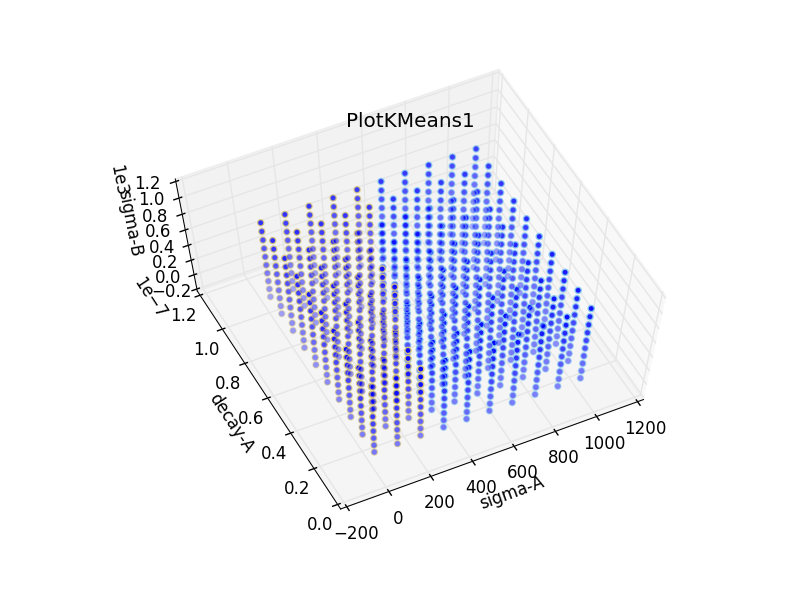
\includegraphics[scale=0.7]{pics/dataminingK-means.png}
  \caption{K-means clustering on original dataset.}
  \label{fig:KmeanOrigData}
 \end{figure}
   \item \textbf{\textit{Steps}}:
\begin{lstlisting}[style=XML,morekeywords={arg,extension,pauseAtEnd,overwrite}]
  <Steps>
    <MultiRun name="sampleMC">
      <Input   class="Files"       type="input">referenceInput.xml</Input>
      <Model   class="Models"      type="Code">testModel</Model>
      <Sampler class="Samplers"    type="Grid">grid</Sampler>
      <Output  class="DataObjects" type="PointSet">samplesMC</Output>
      <Output  class="DataObjects" type="HistorySet">histories</Output>
    </MultiRun>
    <PostProcess name="kmeans" pauseAtEnd="True">
      <Input class="DataObjects" type="PointSet">samplesMC</Input>
      <Model class="Models" type="PostProcessor">KMeans1</Model>
      <Output class="DataObjects" type="PointSet">samplesMC</Output>
      <Output class="OutStreams" type="Plot">PlotKMeans1</Output>
      <Output class="OutStreams" type="Plot">PlotAll</Output>
      <Output class="OutStreams" type="Print">samplesMCdump</Output>
    </PostProcess>
    <PostProcess name="pca" pauseAtEnd="True">
      <Input class="DataObjects" type="PointSet">samplesMC</Input>
      <Model class="Models" type="PostProcessor">PCA1</Model>
      <Output class="DataObjects" type="PointSet">samplesMC</Output>
      <Output class="OutStreams" type="Plot">PlotPCA1</Output>
    </PostProcess>
  </Steps>
\end{lstlisting}

 %%%%%%%%%%%%%%%%%%%%%%%%%%%%%%%%%%%%%%%%%%%%%%%%%%%%%%%%%%
 %%%%%%%%%%%%%%%%%%%%%%%%%%%%%%%%%%%%%%%%%%%%%%%%%%%%%%%%%%
   Finally, all the previously defined \textbf{Entities} can be combined in
   the \xmlNode{Steps} block;
   3 \xmlNode{Steps} have been inputted:
   \begin{itemize}
     \item \xmlNode{MultiRun} named ``sampleMC'', used to run the
     multiple
     instances of the driven code and
     collect the outputs in the two \textit{DataObjects}.The \xmlNode{Sampler} is inputted to communicate to the
     \textit{Step} that the driven code needs to
     be perturbed through the Grid sampling strategy;
     \item \xmlNode{PostProcess} named ``kmeans'', used
     to analyze the data obtained through the sampling strategy. In
     this step, a K-Means algorithm is going to be employed, plotting
     the clustering results;
     \textit{Step} that the driven code needs to
     be perturbed through the Grid sampling strategy;
     \item \xmlNode{PostProcess} named ``pca'', used
     to analyze the data obtained through the sampling strategy. In
     this Step, a PCA algorithm is going to be employed, plotting
     the decomposition results.
   \end{itemize}
\end{enumerate}
Figure~\ref{fig:KmeanOrigData} shows the clustering on the original
input space.
\\Figure~\ref{fig:KmeanProjected} shows the clustering on the projected
input space. It can be noticed, that the algorithm fully capture the fact
that the parameter $sigma-B$ does not impact the response $A$ (being completely independent).
\\Figure~\ref{fig:PCAplot} shows the PCA decomposition on the data set.
%%%%%%%%%%%%%%%%%%%%%%%%%%%%%%%%%%%%%%%%%%%%%%%%%%%%%%%%%%
 %figure samples
 \begin{figure}[h!]
  \centering
  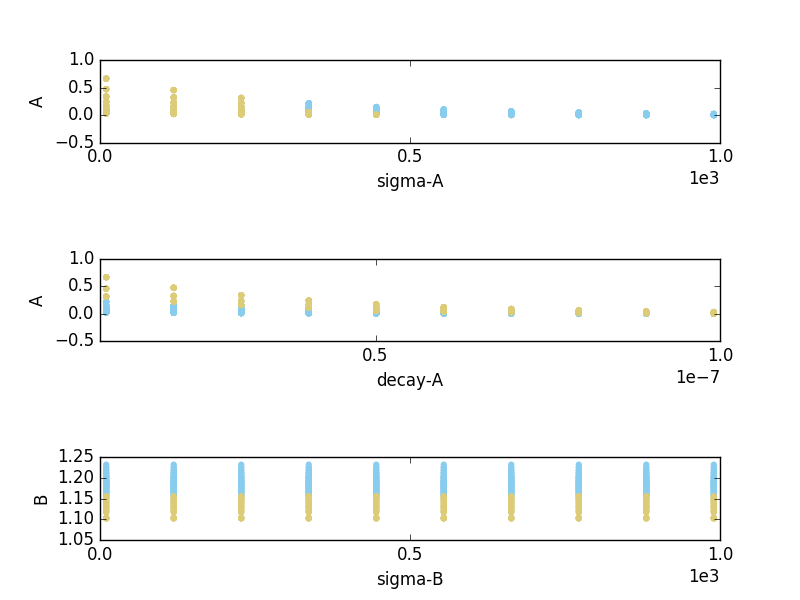
\includegraphics[scale=0.7]{pics/dataminingPlotallK-means.png}
  \caption{K-means clustering on projected parameters.}
  \label{fig:KmeanProjected}
 \end{figure}
 %%%%%%%%%%%%%%%%%%%%%%%%
 %%%%%%%%%%%%%%%%%%%%%%%%%%%%%%%%%%%%%%%%%%%%%%%%%%%%%%%%%%

 %%%%%%%%%%%%%%%%%%%%%%%%
  %%%%%%%%%%%%%%%%%%%%%%%%%%%%%%%%%%%%%%%%%%%%%%%%%%%%%%%%%%
 %figure samples
 \begin{figure}[h!]
  \centering
  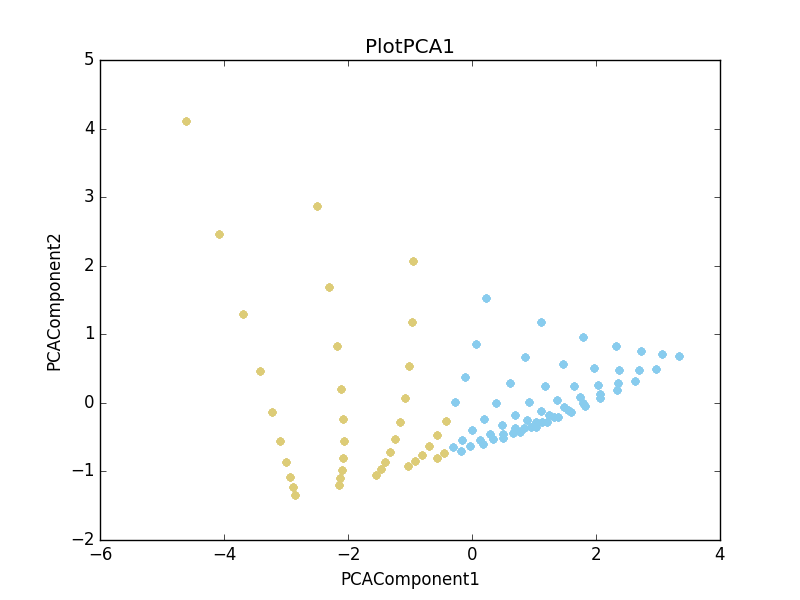
\includegraphics[scale=0.7]{pics/dataminingPCA.png}
  \caption{Principal Component Analysis.}
  \label{fig:PCAplot}
 \end{figure}
 %%%%%%%%%%%%%%%%%%%%%%%%

